\chapter{Cache}

We here continue the discussion on Memory. 

\section{Introduction}
Cache-Main Memory mapping is a way to record which part of the Main Memory is currently in the cache. There are two design concerns: efficiency and effectiveness. We want to make the fast determination of cache hits or misses, and make full use of the cache, which increases the probability of cache hits.

Then, we must answer two questions: how do we know if a data item is in the cache? If it is, how do we find it?

Cache size is much smaller than the main memory size. Thus, a block in the main memory maps to a block in the cache, where both are constructed from many blocks. Since the number of blocks in the cache is smaller than in the main memory, this relationship is called a \textbf{many-to-one mapping}.

\section{Direct Mapping}
One way to perform the mapping is called \textbf{direct mapping}. Here, we consider a main memory address that is 16 bits wide. It is divided into three fields:
\begin{itemize}
  \item \textbf{Cache tag}: occupies 5 bits (values from 0 to 31)
  \item \textbf{Cache block number}: occupies 7 bits (values from 0 to 127)
  \item \textbf{Byte address within the block}: occupies 4 bits
\end{itemize}

Thus, there are in total \(2^4 = 16\) bytes in a block, \(2^7 = 128\) Cache blocks, and \(2^{(7 + 5)} = 4096\) Main Memory blocks.

\begin{minipage}{0.45\textwidth}
The \textbf{Cache tag} is used to identify which \textbf{specific} block from main memory is currently stored in the cache. This is important because many main memory blocks can map to the same position in the cache. The \textbf{Cache Block Number} determines the location of the block in the cache and is used to index the cache. The last few bits of the address select the target word within the block.
\end{minipage}\quad
\begin{minipage}{0.5\textwidth}
  \begin{center}
    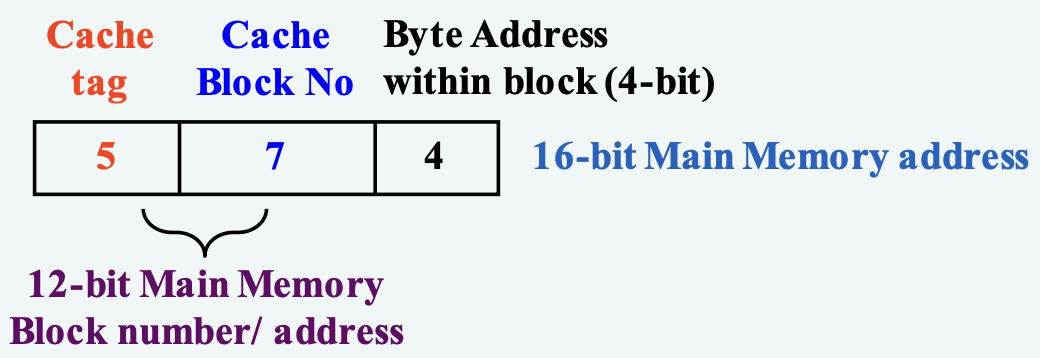
\includegraphics[width=\textwidth]{Figure/direct_mapping.png}
  \end{center}
\end{minipage}

For example, for a block \(j\) of Main Memory, it maps to Block \((j \mod 128)\) of the Cache. A cache hit occurs if the tag matches the desired address. 

One way to understand this is by using a \textbf{hash table} analogy. Many values can hash to the same index. If the desired value is found in the corresponding cache block, it is considered a \textbf{hit}; otherwise, it is a \textbf{miss}.

For a given address \verb|t, b, w|, we can check if it is already in cache by comparing \verb|t| with the tag in block \verb|b|. If the tags do not match, it results in a cache miss. In that case, we replace the current block at \verb|b| with a new one from Memory block \verb|t, b|.

For example, if the CPU is looking for \verb|A7B4|, where MAR = \verb|1010011110110100|, it goes to cache block \verb|1111011| and checks if the tag is \verb|10100|. If so, it's a cache hit. Otherwise, the block is fetched into cache row \verb|1111011|.

In direct mapping, a block in main memory is always mapped to the same cache location. If there is a conflict in address, at most one of them can be mapped to the cache. If a cache block is not mapped, its \texttt{valid} bit is set to 0.

The number of bits includes both the storage for data and for the tags. For a direct-mapped cache with \(2^n\) blocks, \(n\) bits are used for the index. For a block size of \(2^m\) words (\(2^{m+2}\) bytes), \(m\) bits are used to address the word within the block.

2 bits are used to address the byte within the word.

We can also calculate the size of the tag field as follows (for the case that it uses a 32-bit address):
\[
  \text{Tag size} = 32 - (n + m + 2)
\]
The total number of bits in a direct-mapped cache is:
\[
  2^n \times (\text{block size} + \text{tag field size} + \text{valid field size})
\]

The \textbf{Cache tag} is used to identify which \textbf{specific} block from main memory is currently stored in the cache. This is important because many main memory blocks can map to the same position in the cache. The \textbf{Cache Block Number} determines the location of the block in the cache and is used to index the cache. The last few bits of the address select the target word within the block.

Then, for the total number of bits in a direct-mapped cache, we have
\[
  2^{10} \times (4 \times 32 + (32 - 10 - 2 - 2) + 1) = 147\,\text{Kbits}
\]

\begin{remark}
  1 word = 4 bytes = 32 bits
\end{remark}

\section{Associative Mapping}
A Main Memory block can also be in an arbitrary Cache block location. For example, we can divide the 16-bit main memory address into two parts, with the tag occupying 12 bits, and the byte address occupying 4 bits. Then, all 128 tag entries must be compared with the address tag in parallel.

For example, if the CPU is looking for \verb|A7B4|, where MAR = \verb|1010011110110100|, it will check if the tag \verb|101001111011| matches one of the 128 cache tags. If yes, then it's a cache hit. Otherwise, we will load the block into the BINGO cache row.

We can combine the Associative and direct mapping. We again divide the field into 3 parts, where the first 6 bits are the tag, the following 6 bits are the set number, and the last 4 bits are the byte address. We can derive the set number by using \(j \mod 64\), where a cache with \(k\)-blocks per set is called a \(k\)-way set-associative cache.

Again, if the CPU is looking for \verb|A7B4|, where MAR = \verb|1010011110110100|, it goes to check the set \verb|111011|. It will see if one of the two tags in the set \verb|111011| is \verb|101001|. If yes, then it is a cache hit. Otherwise, we will load the block into the BINGO cache row.

For a fixed-size cache, the tag is used to perform tag comparison, the index is used to select the set, and the block offset is used to select the word within the block. For direct mapping, we have smaller tags, but for fully associative mapping, the tag consists of all the bits except the block and byte offsets. This is distinguished by a "freedom line" between the tag field and the index field.

We call it fully associative (with maximum freedom) when each block can be mapped to any location, and to find the block, we need to compare the tag each time we perform a lookup.

\section{Replacement}
When finding a block in the cache, if there is a read hit, that is desirable. However, when there is a read miss, we need to stall the pipeline, fetch the block from the next level in the memory hierarchy, install it in the cache, send the requested word to the processor, and then let the pipeline resume.

Here, we consider only the case when cache write hits. There are two cases:

The first one is \textbf{write-through}, where the cache and memory must remain consistent, and we always write the data into both the cache block and the next level in the memory hierarchy. We can use a write-buffer and stall only when the buffer is full to speed up the process. Notice that memory updates can be handled by the buffer, which operates independently of the processor pipeline. This method is easier to implement. Notice that read misses don't result in writes. 

Another case is \textbf{write-back}. In this method, we write the data only into the cache block, and update the memory hierarchy only when that cache block is \textit{evicted} (replaced). Thus, we need a \textbf{dirty bit} for each data cache block.

\begin{remark}
  A \textbf{dirty bit} is a flag used in cache memory management to track whether the data in a cache block has been modified (written to) since it was last loaded from main memory.
\end{remark}

Here we return to the mapping techniques discussed in the previous sections. For \textbf{direct mapping}, the position of each block is fixed. Whenever replacement is needed (i.e., a cache miss leading to a new block being loaded), the choice is obvious, and thus no replacement algorithm is needed.

However, for \textbf{associative} and \textbf{set-associative} mapping, we need to decide which block to replace, aiming to keep the ones likely to be used again in the near future.

One strategy we can use is the \textbf{Least Recently Used (LRU)} policy. For example, for a 4-block cache, we use a \(\log_2 4 = 2\)-bit counter for each block. We reset the counter to 0 whenever the block is accessed, and the counters of other blocks in the same set are incremented. On a cache miss, we replace (or uncache) a block whose counter reaches 3.

Another strategy we can use is \textbf{random replacement}. We choose a random block to replace, which is easier to implement at high speed.